\documentclass{article}
\usepackage[romanian]{babel}
\usepackage[utf8]{inputenc}
\usepackage{graphicx}
\graphicspath{ {./images/} }

\title{Metode de analiză a circuitelor}
\author{Dinu Mihai Dinel}
\date{}



\begin{document}

\maketitle

\begin{abstract}
Analiza circuitelor, sau rezolvarea circuitelor, înseamnă determinarea tensiunilor și intensităților în fiecare element de circuit. Lucrarea de față își propune să prezinte diferitele metode de analiză de circuit. 
\end{abstract}

\section{Introducere}

\par Un circuit electric/electronic este un sistem compus din elemente electronice, cum ar fi \textbf{rezistențe, tranzistoare, condensatoare, inductori, diode} și multe altele, conectate prin fire prin care poate circula curentul electric.
\par Analiza de circuit este analiza matematică a unui circuit electric sau electronic. Este procesul de studiu și analiză a mărimilor electrice prin calcule. Prin această analiză, putem găsi elementele necunoscute ale unui circuit, cum ar fi \textbf{tensiunea, intensitatea, rezistența, impedanța, puterea}. Când facem analiza circuitelor, trebuie să înțelegem mărimile electrice, relațiile, teoremele și unele legi esențiale.
\par Există două legi esențiale pentru analiza circuitelor. Acestea sunt legile de bază ale rețelei și anume, cele două legi ale lui Kirchhoff:
\par \textbf{Prima lege (sau „Legea nodurilor”)} care enunță că \textit{suma intensităților curenților care intră într-un nod de rețea este egală cu suma intensităților care ies din același nod} și
\par \textbf{A doua lege (sau „Legea ochiurilor”)} care enunță că \textit{de-a lungul conturului unui ochi de rețea, suma algebrică a tensiunilor electromotoare este egală cu suma algebrică a produselor dintre intensitatea curenților și rezistența totală de pe fiecare latură.}

\section{Analiza Nodală}
Analiza nodală oferă o procedură generală pentru analiza circuitelor folosind tensiunile din noduri ca variabile de circuit. Alegerea tensiunilor de pe noduri în detrimentul tensiunilor elementelor ca variabile de circuit este mai convenabilă și reduce numărul de ecuații care trebuie să fie rezolvate simultan.
Pașii de determinare a tensiunilor de pe noduri:
\begin{enumerate}
\item Este selectat un nod ca nod de referință. Sunt atribuite tensiunile \(v1, v2,...,vn-1\) celor n-1 noduri rămase. Tensiunile sunt raportate la nodul de referință.
\item Este aplicată Teorema lui Kirchhoff pentru intensitățile care intră și ies dintr-un nod pe cele n-1 noduri. Este folosită legea lui Ohm pentru a exprima intensitățile pe lature în funcție de tensiunile nodale.
\item Sunt rezolvate ecuațiile rezultante pentru a obține tensiunile necunoscute.
\end{enumerate}


\begin{figure}[h]
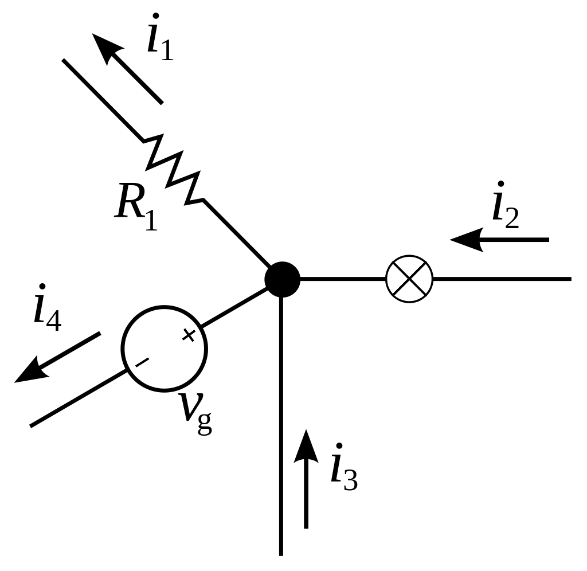
\includegraphics[width=8cm]{fig1.png}
\centering
\caption{Suma intensităților curenților care intră într-un nod de rețea este egală cu suma intensităților curenților care ies din același nod. \(i1 + i4 = i2 + i3\)}
\end{figure}

\par Prima lege a lui Kirchhoff:
\[\sum_{}^{}i_{k}=0\]

\section{Analiza Ochiurilor}
\par Analiza ochiurilor oferă o altă procedură generală pentru analizarea circuitelor, utilizând curenții rețelei ca variabile ale circuitului. Utilizarea curenților din ochiuri în loc de curenții elementelor ca variabile de circuit este convenabilă și reduce numărul de ecuații care trebuie rezolvate simultan.
\par Amintiți-vă că o buclă este o cale închisă fără un nod trecut de mai multe ori. Un ochi este o buclă care nu conține nicio altă buclă în ea.
\par Analiza nodală aplică Teorema lui Kirchhoff pentru intensități pentru a găsi tensiuni necunoscute într-un circuit dat, în timp ce analiza rețelei aplică Teorema lui Kirchhoff pentru tensiuni pentru a găsi curenții necunoscuți.
\par Analiza rețelei nu este la fel de generală ca analiza nodală, deoarece este aplicabilă numai unui circuit planar. Un circuit plan este unul care poate fi desenat într-un plan fără ramuri care se încrucișează; altfel este neplanar. Un circuit poate avea ramuri care se încrucișează și să fie totuși plan dacă poate fi redesenat astfel încât să nu aibă ramuri care se încrucișează.
\par Pașii de determinare:
\begin{enumerate}
\item Sunt atribuiți curenții de ochiuri i1, i2, ...,in celor n ochiuri.
\item Este aplicată Teorema lui Kirchhoff pentru tensiuni pe cele n ochiuri. Este folosită legea lui Ohm pentru a exprima tensiunile în funcție de intensități.
\item Sunt rezolvate ecuațiile rezultante pentru a obține tensiunile din ochiuri.
\end{enumerate}


\begin{figure}[h]
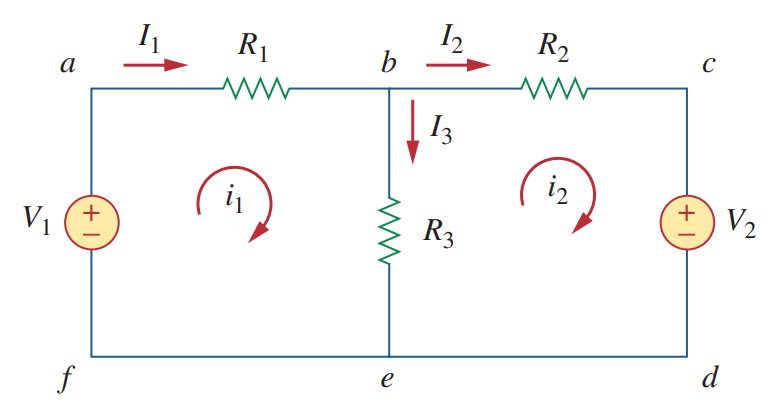
\includegraphics[width=8cm]{fig2.png}
\centering
\end{figure}

\par A doua lege a lui Kirchhoff:
\[\sum E_n=\sum{R_nI_n}\]
\[\sum V_n=0\]


\section{Concluzii}
Din cele prezentate anterior, observam ca metodele de analiza a ochiurilor sunt ușor de aplicat, iar asta reprezintă un avantaj important, ce poate însemna, printre altele, ca pot fi implementate ușor în programe de calculator care sa automatizeze acest proces.


\section{Bibliografie}
\begin{enumerate}
    \item Legile lui Kirchhoff – Wikipedia
    \item Fundamentals of Electric Circuits – Charles K. Alexander and Matthew
\end{enumerate}

\end{document}

